\documentclass{article}
\usepackage{tmlr}

% === Packages ===
\usepackage{amsmath, amssymb}
\usepackage{booktabs}
\usepackage{graphicx}
\usepackage{hyperref}
\usepackage{xcolor}
\usepackage{enumitem}
\usepackage{tikz}
\usetikzlibrary{arrows.meta, positioning}

\title{Benchmarks Are Engines, Not Cameras:\\Performativity, Proof Cultures, and the Social Production\\of Machine Learning Knowledge}

\author{Anonymous}

\def\month{06}
\def\year{2026}

\begin{document}
\maketitle

% ============================================================
% ABSTRACT
% ============================================================
\begin{abstract}
Machine learning benchmarks function as engines, not cameras: they reshape the practices they measure rather than passively recording them. Drawing on MacKenzie's sociology of financial models, we document three mechanisms by which benchmarks produce ML knowledge. First, benchmark adoption and abandonment tracks social utility rather than scientific exhaustion---NLP benchmarks complete their lifecycle in 3--5 years; vision benchmarks persist for 10+. Second, mechanistic interpretability subfields operate with incommensurable proof standards for equivalent claims; citation cross-density between SAE and causal-abstraction communities is 1.4\%, despite shared foundational roots. Third, reviewer experiment demands introduce implicit comparisons without adjustment---a pattern we call counterperformative peer review. Using citation analysis of benchmark lifecycle curves via OpenAlex, a manual comparison-count audit of 18 papers (12 landmark ML, 6 mechanistic interpretability), and demand-compliance analysis of 11,196 ICLR submissions across 2023--2024, we find: (i)~the median landmark paper contains 414 implicit comparisons, of which 11/12 papers report zero corrections; (ii)~statistical correction adoption is not merely low but \emph{declining}---Benjamini-Hochberg citations fell from 0.17\% to 0.09\% of ML output between 2019 and 2025; and (iii)~the aggregate compliance--acceptance association ($+$10.7\,pp in 2024, $+$13.0\,pp in 2023) is a Simpson's paradox concentrated in borderline-scored papers ($+$2.9\,pp, $n=53$), precisely the stratum where selective reporting is most consequential. The central argument is not that ML researchers are individually careless, but that the evaluation culture's instruments both measure and manufacture what counts as knowledge---and that statistical reforms alone cannot address causes that are sociological.
\end{abstract}

% ============================================================
% 1. INTRODUCTION
% ============================================================
\section{Introduction}
\label{sec:intro}

In 2006, MacKenzie argued that financial models are better understood as \textit{engines} that reshape markets than as \textit{cameras} that passively record them~\citep{mackenzie_engine_2006}. The Black-Scholes options-pricing model did not merely describe prices; traders adopted it, and prices came to conform to it---a phenomenon MacKenzie termed \textit{Barnesian performativity}~\citep{mackenzie_millo_2003}. The model made itself true.

We argue that the same dynamic operates in machine learning research, with benchmarks playing the role of pricing models. ImageNet~\citep{deng_imagenet_2009} does not passively measure visual understanding; it defines what visual understanding \textit{means} for the research community, shapes training procedures, data collection, and career incentives, and is abandoned not when vision is ``solved'' but when a new benchmark captures the community's attention. GLUE~\citep{wang_glue_2018} did not measure natural language understanding; it measured the ability to fine-tune on a specific task distribution, and was replaced by SuperGLUE within two years. MMLU~\citep{hendrycks_mmlu_2021} measures test-taking on multiple-choice questions at least as much as it measures reasoning, and is already being supplemented by benchmarks that its own creators argue more faithfully capture what MMLU was supposed to.

The benchmark is an engine, not a camera. And like the Gaussian copula whose widespread adoption created correlated fragility it could not represent~\citep{mackenzie_bamford_2018}, widespread optimisation against a benchmark can create overfitting it cannot detect---because the benchmark is the detection instrument.

\paragraph{A clarification on framing.} Throughout this paper, we use the language of multiple comparisons and family-wise error rates (FWER) as a diagnostic tool. We are not claiming that ML researchers are secretly performing null-hypothesis significance tests. Most ML papers do not compute $p$-values at all. Our argument is narrower: when a researcher trains 50 configurations and reports the best one, the reported performance is inflated by selection on noise---the winner's curse from order statistics---and Bonferroni thresholds provide a convenient upper bound on this inflation. The selection effect operates regardless of whether a $p$-value is computed.

\paragraph{Contributions.} Using a manual comparison-count audit of 18 papers, citation-based analysis of 8 benchmark lifecycle curves and statistical correction adoption rates via OpenAlex~\citep{priem_openalex_2022}, and demand-compliance analysis of 11,196 ICLR submissions across 2023--2024, we document three linked mechanisms:

\begin{enumerate}[leftmargin=*]
\item \textbf{Benchmark performativity cycles} (Section~\ref{sec:performativity}): adoption and abandonment tracks social utility, not scientific exhaustion; NLP benchmarks complete this cycle in 3--5 years, vision benchmarks in 10+.
\item \textbf{Proof-culture fragmentation} (Section~\ref{sec:proof_cultures}): in mechanistic interpretability, SAE and causal-abstraction communities accept incommensurable forms of evidence for equivalent claims; cross-community citation density is 1.4\%.
\item \textbf{Counterperformative peer review} (Section~\ref{sec:counterperformativity}): reviewer experiment demands introduce new implicit comparisons; the aggregate compliance--acceptance association is a Simpson's paradox concentrated in borderline submissions where selective reporting is most tempting.
\end{enumerate}

ML's evaluation failures are better understood as structural rather than individual: the publication system preferentially admits novel positive results and makes it structurally difficult to publish the replications, null findings, and modest corrections that would surface false positives.

% ============================================================
% 2. THEORETICAL FRAMEWORK
% ============================================================
\section{Theoretical Framework}
\label{sec:theory}

We draw on three strands of work from the sociology of science that have not previously been applied to ML evaluation methodology.

\subsection{Performativity}

MacKenzie~\citep{mackenzie_engine_2006} distinguishes three levels of performativity:

\begin{description}[leftmargin=1.5cm]
\item[Generic] Practitioners use a theory or model in their work.
\item[Effective] Use of the theory has a causal effect on the phenomenon it describes.
\item[Barnesian] Use of the theory makes the world conform more closely to the model---the strongest form, in which the map redraws the territory.
\end{description}

He also introduced, with Bamford, the concept of \textit{counterperformativity}: when a model's widespread adoption causes the world to \emph{diverge} from the model's predictions---as when universal use of the Gaussian copula in credit risk created the very correlations the model assumed away~\citep{mackenzie_bamford_2018}.

For ML benchmarks, we claim \textit{effective} performativity, not Barnesian: benchmarks causally reshape research priorities, training procedures, and career incentives, but we do not claim that the world comes to conform to the benchmark's implicit model in the strong sense that options prices came to conform to Black-Scholes. The closest analogy is Espeland and Sauder's~\citep{espeland_sauder_2007} analysis of law school rankings, where rankings reshaped admissions criteria, resource allocation, and strategic behaviour without making law schools conform to an underlying formal model.

The distinction between performativity and Goodhart's Law~\citep{goodhart_1975} is substantive. Goodhart describes the \textit{symptom}: measures captured by their use. Performativity theory describes the \textit{mechanism}: which institutional channels sustain the degradation, why it is self-reinforcing, and how counterperformativity creates the specific failure mode in which the safety apparatus generates the risk it was designed to prevent. Our ICLR data (Section~\ref{sec:counterperformativity}) provide empirical evidence for counterperformativity in the peer review system itself.

\subsection{Cultures of Proving}

In his work on formal verification, MacKenzie showed that what counts as a valid ``proof'' is not a settled logical matter but a socially negotiated boundary---logicians, mathematicians, and engineers accepted different kinds of arguments as proof, with closure shaped by funding structures and regulatory demands~\citep{mackenzie_mechanizing_2001}. Section~\ref{sec:proof_cultures} applies this framework to mechanistic interpretability, where at least three communities have developed incommensurable proof standards for what constitutes a valid mechanistic claim.

\subsection{Publication Bias and Structural Selection}

The replication crisis literature has documented three stacked asymmetries in the publication system~\citep{franco_publication_2014, simonsohn_p_curve_2014}:

\begin{enumerate}[leftmargin=*]
\item \textbf{Positive-results bias.} Journals overwhelmingly accept positive, novel findings; null results are not published.
\item \textbf{Anti-replication bias.} Reviewers treat replication studies as ``not novel'' regardless of their scientific value.
\item \textbf{Gotcha bias.} Disproofs are publishable only when they dramatically overturn a famous result---modest corrections are rejected as ``not surprising.''
\end{enumerate}

Together, these create a one-sided filter: the very outputs that would correct the literature's false-positive accumulation are the outputs the system tends to reject.

% ============================================================
% 3. DATA AND METHODS
% ============================================================
\section{Data and Methods}
\label{sec:methods}

\subsection{OpenReview Demand-Compliance Analysis}

We analysed all publicly available submissions to ICLR 2024 ($n = 7{,}404$) and ICLR 2023 ($n = 3{,}792$), retrieved via the OpenReview REST API. For each submission, we extracted: (i)~explicit experiment demands from reviewer text using keyword patterns (Appendix~\ref{app:iclr_method}); (ii)~author compliance signals from rebuttals; and (iii)~final acceptance decisions and mean reviewer scores. The extraction pipeline achieved 84\% agreement with manual labelling on a 50-paper subsample; the disagreements were approximately equally split between false positives (demand language in non-demand context) and false negatives (implicit compliance not signalled in rebuttal text), so the direction of bias is not clear. We note that this is an observational study: papers that comply may differ systematically from those that do not (e.g., in lab resources, initial paper quality, or English proficiency). Score-stratified analysis (Table~\ref{tab:stratified}) controls for the most salient confounder, but residual confounding cannot be excluded.

\subsection{OpenAlex Citation Analysis}

We use structured citation metadata from OpenAlex~\citep{priem_openalex_2022} to track two trends via citation links, not keyword matching: (i)~benchmark lifecycle curves, measuring year-by-year citation counts for 8 major benchmark-introducing papers; and (ii)~statistical correction adoption rates, measuring the fraction of ML papers per year that cite the canonical papers introducing Bonferroni~\citep{dunn_1961}, Holm~\citep{holm_1979}, or Benjamini-Hochberg~\citep{benjamini_hochberg_1995} corrections. The ML paper population is defined as works tagged with the ``Machine learning'' concept in OpenAlex.

\subsection{Manual Comparison-Count Audit}

We conducted a manual audit of implicit comparisons in 12 landmark ML papers and 6 mechanistic interpretability papers (Appendices~\ref{app:landmark_audit} and~\ref{app:mi_audit}). For each results table, we count pairwise row comparisons within each metric column---a lower bound, since unreported hyperparameter sweeps and preliminary experiments are not captured. For MI papers, we additionally record the total dictionary size ($N$), the number of features deeply examined ($k$), and the implied Bonferroni threshold on total comparisons.

\subsection{Cross-Community Citation Analysis}

To quantify proof-culture fragmentation in mechanistic interpretability (Section~\ref{sec:proof_cultures}), we assembled a corpus of 27 canonical MI papers across three communities (SAE, causal abstraction, and circuit discovery; 2020--2025), retrieved via Semantic Scholar and OpenAlex APIs. We computed cross-community citation density as the fraction of directed citation pairs between non-overlapping communities that were actually realised. The sample captures canonical papers; the full MI literature may show denser cross-citation at the periphery. Temporal asymmetry (circuits papers predate SAE and causal-abstraction work) explains the absence of reverse citations from circuits to newer communities.

\subsection{Prospective File-Drawer Log}

During development, we maintained a prospective comparison log---a running record of all analyses attempted but not included in the final paper. The log is reproduced in part in Section~\ref{sec:discussion} as a concrete illustration of the file-drawer problem we document. To our knowledge, this is the first prospective comparison log published alongside an ML empirical study.

% ============================================================
% 4. BENCHMARKS AS ENGINES
% ============================================================
\section{Benchmarks as Engines}
\label{sec:performativity}

\subsection{The Performativity Cycle}

We observe a recurring four-phase cycle in benchmark adoption:

\begin{enumerate}[leftmargin=*]
\item \textbf{Introduction (camera phase).} A benchmark is proposed as a measurement instrument. At introduction, it functions as a camera: it passively records model performance.
\item \textbf{Adoption (generic performativity).} Researchers begin optimising against the benchmark. Leaderboards emerge. The benchmark's scores become the operational definition of the capability it was designed to measure.
\item \textbf{Saturation (effective performativity).} Optimisation changes training procedures, data collection, and architecture choices. The benchmark has a causal effect on the phenomenon: models get better \textit{at the benchmark}, which may or may not correspond to improvement in the underlying capability. Transfer studies (e.g., \citealt{recht_imagenet_2019}) begin revealing the gap.
\item \textbf{Abandonment or replacement (counterperformativity).} The benchmark is either saturated (human-level accuracy renders further comparison meaningless) or recognised as no longer measuring what it was supposed to. A new benchmark is introduced, and the cycle restarts.
\end{enumerate}

Citation-based lifecycle data from OpenAlex (Table~\ref{tab:lifespans}) confirm that NLP benchmarks complete this cycle faster than vision benchmarks. GLUE peaked in 2023 at 1,052 citations per year and dropped 54\% by 2024; SuperGLUE peaked the same year and dropped 69\%. ImageNet peaked in 2021 at 9,305 citations per year but declined only 16\% by 2024, sustained by its role as a pretraining dataset and cultural reference point.

\begin{table}[t]
\centering
\caption{Benchmark performativity cycles, measured by year-over-year citation counts from OpenAlex. Decline is measured from peak year to 2024. NLP benchmarks complete the camera$\to$engine transition in 3--5 years; vision benchmarks persist for 10+. Citation counts conflate usage and critique; we report them as evidence of shifting community attention, not as proof of abandonment.}
\label{tab:lifespans}
\small
\begin{tabular}{@{}lccrrc@{}}
\toprule
Benchmark & Domain & Intro & Peak year & Peak cites/yr & Decline to 2024 \\
\midrule
GLUE & NLP & 2018 & 2023 & 1{,}052 & $-$54\% \\
SuperGLUE & NLP & 2019 & 2023 & 359 & $-$69\% \\
SQuAD & NLP & 2016 & 2021 & 1{,}237 & $-$59\% \\
\midrule
ImageNet & Vision & 2009 & 2021 & 9{,}305 & $-$16\% \\
CIFAR-10 & Vision & 2009 & 2021 & 4{,}870 & $-$39\% \\
\midrule
MMLU & LLM & 2021 & 2023 & 133 & $-$24\% \\
HumanEval & Code & 2021 & 2023 & 604 & $-$35\% \\
HELM & LLM & 2022 & 2023 & 146 & $-$15\% \\
\bottomrule
\end{tabular}
\end{table}

\subsection{Counterperformativity: When Benchmarks Break}

The counterperformative moment has a specific signature in ML: the benchmark is revealed to be testing something other than what it is named after. MMLU tests multiple-choice test-taking, not ``massive multitask language understanding.'' GLUE tested fine-tuning ability, not ``general language understanding.'' The name persists after the measurement has diverged, creating a sustained gap between what the community says it is measuring and what it is measuring.

This is the Gaussian copula dynamic transplanted into research evaluation. Widespread optimisation against a benchmark can create overfitting the benchmark itself cannot detect, because the benchmark \textit{is} the detection instrument. The solution---a new benchmark---restarts the cycle rather than resolving it.

% ============================================================
% 5. PROOF CULTURES AND THEIR FRAGMENTATION
% ============================================================
\section{Proof Cultures and Their Fragmentation}
\label{sec:proof_cultures}

\subsection{Three Proof Cultures in Mechanistic Interpretability}

The emerging subfield of mechanistic interpretability (MI)---the attempt to reverse-engineer the internal computations of neural networks---provides a particularly clear case of proof-culture fragmentation. We identify three communities operating with distinct and largely incommensurable standards for what constitutes a valid mechanistic claim:

\begin{description}[leftmargin=*]
\item[Sparse autoencoders (SAE).] Validity is established by demonstrating that learned features are monosemantic, sparse, and reconstructive of model activations. The proof standard is \textit{feature-level}: a mechanism is valid if its component features are interpretable. The persuasive object is a feature dashboard---activating examples, a natural-language label, and a sparse set of tokens that make the feature feel semantically coherent.
\item[Causal abstraction.] Validity is established by showing that an interpretive model is causally aligned with the neural network under interchange interventions~\citep{geiger_causal_2021}. The proof standard is \textit{intervention-level}: a mechanism is valid if intervening on the proposed variables produces the predicted effect on behaviour. The persuasive object is an intervention result.
\item[Circuit discovery.] Validity is established by identifying subgraphs of the network that are sufficient to reproduce behaviour on a task, via activation patching or edge attribution. The proof standard is \textit{sufficiency-level}: a mechanism is valid if the identified circuit is sufficient and necessary for the behaviour. The persuasive object is a subgraph.
\end{description}

These are not merely different methods; they reflect different ontological commitments about what a ``mechanism'' is. The SAE community treats mechanisms as collections of features. The causal abstraction community treats them as causal models. The circuit community treats them as computational subgraphs.

\subsection{Empirical Evidence of Fragmentation}

A citation analysis of 27 canonical MI papers across the three communities confirms the fragmentation empirically. SAE and causal-abstraction papers share only 1 cross-citation across 72 possible directed paper pairs---a cross-community density of 1.4\%---despite both communities citing the foundational circuit-discovery literature heavily (19 combined edges). The pattern is two newer proof cultures building independently on the same older foundation without citing each other.

The fragmentation becomes visible in what each community treats as a persuasive figure. A feature dashboard---striking, nameable, emotionally vivid---does not constitute evidence in a causal-abstraction paper. An interchange intervention result does not appear in SAE papers. These evidential forms are not interchangeable because they make different kinds of objects visible and leave different kinds of uncertainty in the background. A circuit diagram says nothing about whether individual features are monosemantic; a feature dashboard says nothing about whether the features causally produce the behaviour.

\subsection{The Social Production of Fragmentation}

Why don't these communities converge? The interdisciplinarity literature suggests an answer: convergence is structurally disincentivised. Junior researchers face career risk from interdisciplinary work~\citep{leahey_prominent_2017}. Grant proposals include other perspectives only superficially~\citep{klein_interdisciplinarity_2010}. The reward structure makes monodisciplinary specialisation the dominant strategy even when the problem demands range~\citep{epstein_range_2019}.

The result is that proof-culture fragmentation is not a temporary state awaiting the right unifying experiment. The incentive structure suggests it may be self-sustaining---maintained by the same publication and career incentives that drive the evaluation culture's other pathologies. MacKenzie's Strong Programme analysis applies: the \textit{content} of mechanistic interpretability knowledge (fragmented, with plural proof standards) is causally shaped by the \textit{social conditions} of its production.

\subsection{The Denominator Problem}
\label{sec:denominator}

The SAE proof culture introduces a distinctive and largely unrecognised selection problem. A sparse autoencoder trains a dictionary of $N$ features (typically $N = 4{,}096$ to $34{,}000{,}000$), each of which is implicitly examined for interpretability. The researcher reports the $k \ll N$ that appear most interesting as evidence that the method ``finds interpretable features.'' This is selection from a large pool on the outcome variable---apparent interpretability---and the denominator is never reported.

A manual FWER audit of six MI papers (Appendix~\ref{app:mi_audit}) finds implied comparisons ranging from 12,000 (Bricken et al.~2023, dictionary of 4,096) to 170,000,000 (Templeton et al.~2024, dictionary of 34M). The Bonferroni threshold for the largest case is $\alpha^* = 2.9 \times 10^{-10}$; no interpretability metric in the literature comes close. Again: we are not claiming these papers perform hypothesis tests. We are using Bonferroni thresholds as a diagnostic for how much the selection ratio should reduce confidence in the claims.

\paragraph{The Bolukbasi--Gonen episode as a cross-field precedent.} The denominator problem is not unique to SAEs. Bolukbasi et al.~\citep{bolukbasi_man_2016} evaluated word-embedding debiasing on the analogy task used to \textit{define} the gender direction---the metric was constructed from the same distribution the debiasing was applied to. The method accumulated 2,685+ citations and was adopted as a preprocessing step before Gonen and Goldberg~\citep{gonen_lipstick_2019} showed via clustering and classifier recovery that the bias was geometrically intact: the debiasing had removed the projection most visible to the original evaluation while leaving relational structure untouched. The failure mode is identical to SAE denomination selection---evaluating on the cases the method was optimised to handle, and treating success there as evidence for the full claim.

\paragraph{SAEBench and coverage.} Recent tools make rate-reporting tractable. SAEBench~\citep{karvonen_saebench_2025} scores each latent by asking an LLM to identify activating sequences from a feature description, yielding scores between 0 and 1. On a Pythia-70M SAE (100 randomly sampled latents), the mean score is 0.84 (SD = 0.12). At production scale, a different failure mode appears: Paulo et al.~\citep{paulo_autointerp_2024} scored millions of features on a 131K-feature Gemma-2 9B SAE and found that 30\% of features do not activate frequently enough to generate the examples the scoring method requires. This is a coverage problem, not a low-interpretability problem. The two failure modes compound: features that activate may score well; features that rarely activate are unmeasurable; published interpretability rates reflect only the former.

\paragraph{Seed instability.} Paulo and Belrose~\citep{paulo_belrose_seeds_2026} showed that SAEs trained on the same model and data with different random seeds learn fundamentally different features: in a 131K-latent SAE on Llama~3 8B, only 30\% of features were shared across seeds. As they conclude, ``the set of features uncovered by an SAE should be viewed as a pragmatically useful decomposition of activation space, rather than an exhaustive and universal list of features `truly used' by the model.'' The reported features are a selected subset of an unstable decomposition---the denominator is not merely large but indeterminate.

\paragraph{The file drawer made visible.} The de facto research methodology in MI---described explicitly by one of the field's leading practitioners as ``Explore $\to$ Understand $\to$ Distill''~\citep{nanda_research_process_2023}---structurally guarantees a file-drawer problem. The exploration stage is explicitly designed not to appear in the written output. A rare exception illustrates the mechanism by contrast: the Google DeepMind MI team published a blog post of research explicitly ``not consider[ed] a good fit for turning into a paper''~\citep{smith_gdm_negative_2025}, reporting negative results from SAE research---failed out-of-distribution probing, absorption, missing features, low sensitivity. Under the standard publication filter, all of this would have remained invisible.

% ============================================================
% 6. THE COUNTERPERFORMATIVITY OF PEER REVIEW
% ============================================================
\section{The Counterperformativity of Peer Review}
\label{sec:counterperformativity}

\subsection{The Mechanism}

The publication system introduces a final counterperformative dynamic. Reviewers, acting in good faith, demand additional experiments: ``run three more seeds,'' ``add two baselines,'' ``test on another dataset.'' Each demand is intended to reduce the false-positive rate. But each demanded experiment is a new fork in the garden of forking paths~\citep{gelman_garden_2013}---a fresh implicit comparison whose result will be selectively reported (the paper is revised to incorporate only the experiments that support the claim).

The mechanism by which this could inflate false positives is straightforward: each demanded experiment increases the implicit comparison count without any corresponding correction. Whether this mechanism operates at scale is an empirical question we cannot definitively answer with observational data. But the structural conditions for it are present, and we now show that the demand-compliance exchange is concentrated precisely where the incentive to comply selectively is highest.

\subsection{Empirical Evidence: The Demand-Compliance Pipeline at ICLR}

Table~\ref{tab:demand_compliance} presents the aggregate results for ICLR 2024 and 2023. In both years, papers that comply with reviewer experiment demands are accepted at higher rates than papers that receive demands but do not comply: $+$10.7\,pp in 2024, $+$13.0\,pp in 2023.

\begin{table}[t]
\centering
\caption{Demand--compliance--outcome pipeline at ICLR (aggregate). The compliance lift replicates across years: $+$10.7\,pp in 2024, $+$13.0\,pp in 2023. This aggregate finding is a Simpson's paradox; see Table~\ref{tab:stratified}.}
\label{tab:demand_compliance}
\small
\begin{tabular}{@{}lrrrr@{}}
\toprule
& \multicolumn{2}{c}{ICLR 2024 ($n = 7{,}404$)} & \multicolumn{2}{c}{ICLR 2023 ($n = 3{,}792$)} \\
\cmidrule(lr){2-3} \cmidrule(lr){4-5}
Condition & Papers & Accept\% & Papers & Accept\% \\
\midrule
No demands received & 5{,}063 & 39.7\% & 3{,}435 & 41.9\% \\
Demands received & 717 & 34.9\% & 357 & 37.3\% \\
\quad Complied & 177 & 42.9\% & 78 & 47.4\% \\
\quad Did not comply & 540 & 32.2\% & 279 & 34.4\% \\
\midrule
Compliance lift & \multicolumn{2}{c}{$+$10.7\,pp} & \multicolumn{2}{c}{$+$13.0\,pp} \\
\bottomrule
\end{tabular}
\end{table}

\subsection{Score Stratification: A Simpson's Paradox}

Table~\ref{tab:stratified} stratifies the same data by mean reviewer score. Within score strata, the lift is small, absent, or reversed:

\begin{itemize}[leftmargin=*]
\item \textbf{Low-scored papers} ($< 4.5$): 0\% acceptance regardless of compliance.
\item \textbf{Borderline papers} (4.5--5.5): $+$2.9\,pp lift for compliant authors ($n = 53$); this is the only stratum with a positive signal.
\item \textbf{Mid-scored papers} (5.5--6.5): compliant authors accepted at \textit{lower} rates ($-$4.7\,pp).
\item \textbf{High-scored papers} ($\geq 6.5$): 94--95\% acceptance regardless.
\end{itemize}

The aggregate lift arises because compliant papers are disproportionately borderline: reviewers issue experiment demands when they are uncertain, and those borderline authors who signal compliance are tipped across the threshold. Non-compliant papers are more concentrated in the low stratum where nothing helps.

\begin{table}[t]
\centering
\caption{Score-stratified demand--compliance analysis (ICLR 2024, $n = 5{,}780$ matched with reviewer scores). The aggregate $+$10.7\,pp compliance lift is a Simpson's paradox: within score strata, the lift is small (borderline), absent (low, high), or negative (mid). Compliant papers are disproportionately borderline; non-compliant papers are disproportionately low-scored.}
\label{tab:stratified}
\small
\begin{tabular}{@{}lccc@{}}
\toprule
Score stratum & Comply accept\% & No-comply accept\% & Lift \\
\midrule
Low ($< 4.5$) & 0.0\% ($n = 15$) & 0.0\% ($n = 155$) & 0.0\,pp \\
Borderline (4.5--5.5) & 7.5\% ($n = 53$) & 4.7\% ($n = 150$) & $+$2.9\,pp \\
Mid (5.5--6.5) & 50.0\% ($n = 70$) & 54.7\% ($n = 139$) & $-$4.7\,pp \\
High ($\geq 6.5$) & 94.9\% ($n = 39$) & 94.8\% ($n = 96$) & $+$0.1\,pp \\
\midrule
Aggregate & 42.9\% ($n = 177$) & 32.2\% ($n = 540$) & $+$10.7\,pp \\
\bottomrule
\end{tabular}
\end{table}

\paragraph{What this does and does not show.} The borderline-stratum signal ($+$2.9\,pp, $n = 53$) is small and compatible with a mundane explanation: compliant borderline papers may be better-resourced or simply better papers. The data cannot distinguish selective reporting from genuine evidential improvement. What the data \textit{do} show is a structural pattern: the compliance incentive concentrates where selective reporting would be most consequential, and the demanded experiments are introduced without any framework for adjusting the comparison count. The replication across two years of the same venue suggests the pattern is stable, not an artefact of a single cohort.

\begin{figure}[t]
\centering
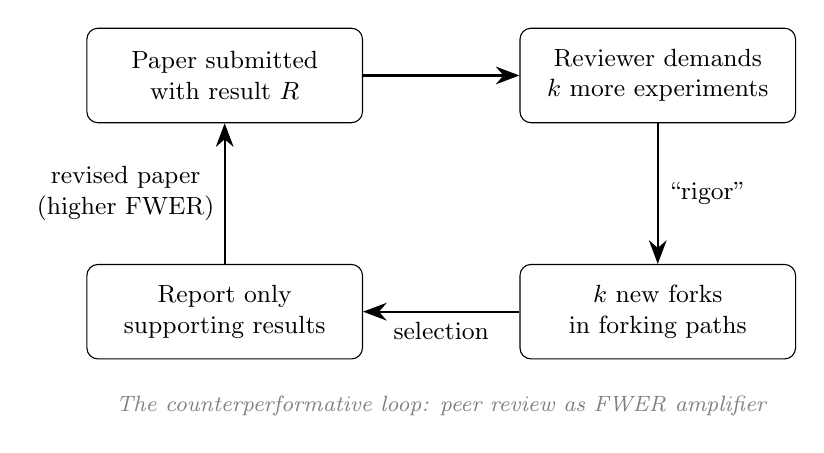
\begin{tikzpicture}[
box/.style={draw, rounded corners, minimum width=3.5cm, minimum height=1.2cm, align=center, font=\small},
arr/.style={-{Stealth[length=3mm]}, thick},
every node/.style={font=\small}
]
\node[box] (submit) at (0,0) {Paper submitted\\with result $R$};
\node[box] (review) at (5.5,0) {Reviewer demands\\$k$ more experiments};
\node[box] (fork) at (5.5,-3) {$k$ new forks\\in forking paths};
\node[box] (select) at (0,-3) {Report only\\supporting results};
\draw[arr] (submit) -- (review);
\draw[arr] (review) -- node[right] {``rigor''} (fork);
\draw[arr] (fork) -- node[below] {selection} (select);
\draw[arr] (select) -- node[left, align=center] {revised paper\\(higher FWER)} (submit);
\node[font=\footnotesize\itshape, text=gray] at (2.75, -4.2) {The counterperformative loop: peer review as FWER amplifier};
\end{tikzpicture}
\caption{Structural conditions for counterperformativity in peer review. Each cycle of reviewer-demanded experiments increases the number of implicit comparisons without comparison-count adjustment. Our ICLR analysis shows that the compliance--acceptance association concentrates in the borderline score stratum, where the incentive for selective reporting is strongest. The data show the structural conditions; whether the mechanism inflates false positives in practice is not directly observable from observational data.}
\label{fig:loop}
\end{figure}

% ============================================================
% 7. THE SELECTION INFLATION PROBLEM
% ============================================================
\section{How Large Is the Selection Inflation?}
\label{sec:inflation}

\subsection{Comparison-Count Audit}

Table~\ref{tab:fwer_audit} in Appendix~\ref{app:landmark_audit} presents a manual audit of 12 landmark ML papers. The median paper contains 414 implicit comparisons from published results tables alone---a lower bound, since unreported hyperparameter sweeps and preliminary experiments are not captured. Of the 12 papers, 11 (92\%) mention zero multiple comparison corrections. The lone exception (CLIP) mentions correction in the context of one experiment, not as a systematic practice across its 58,632 comparisons.

\subsection{Quantifying the Inflation}

From order statistics: if you pick the best of $N$ independent draws from noise with standard deviation $\sigma$, the winner's expected inflation is approximately $\sigma\sqrt{2 \ln N}$. At $N = 414$, that is roughly $3.5\sigma$. But the i.i.d.\ assumption overstates the case---hyperparameter configurations within a paper are correlated (same dataset, overlapping architectures, shared training infrastructure), so the effective number of independent comparisons $N_{\text{eff}}$ may be much smaller. For sensitivity: at $N_{\text{eff}} = 40$, expected inflation drops to $\approx 2.7\sigma$; at $N_{\text{eff}} = 10$, to $\approx 2.1\sigma$. The direction is unambiguous; the magnitude is unknowable without the denominator---which is why reporting comparison counts matters.

From information theory: reporting $k$ results from $N$ candidates discards $\log_2\binom{N}{k}$ bits about the search. For the median paper ($N = 414$, $k \approx 15$ key results), that is roughly 80 bits---the entropy of 80 coin flips. The reader sees the outcomes; the process that selected them is gone.

\subsection{Statistical Correction Adoption Is Declining}

Figure~\ref{fig:correction_trends} plots ML paper citation rates for the three canonical correction papers from 2015 to 2025. Correction adoption is not merely low but \textit{declining} as a fraction of total ML output: Benjamini-Hochberg~\citep{benjamini_hochberg_1995} citations dropped from 0.17\% of ML papers in 2019 to 0.09\% in 2025; Holm~\citep{holm_1979} from 0.06\% to 0.01\%; Bonferroni~\citep{dunn_1961} from 0.03\% to 0.01\%. The statistical corrections exist; the field is not adopting them, and the trend is negative. This is not a knowledge gap---it is a structural selection pressure that makes correction invisible to the reward system.

\begin{figure}[t]
\centering
\begin{tikzpicture}
\begin{axis}[
  width=0.85\textwidth,
  height=5cm,
  xlabel={Year},
  ylabel={Fraction of ML papers (\%)},
  xmin=2015, xmax=2025,
  ymin=0, ymax=0.22,
  xtick={2015,2017,2019,2021,2023,2025},
  legend pos=north east,
  grid=both,
  grid style={line width=0.3pt, draw=gray!30},
  tick label style={font=\small},
  label style={font=\small},
  legend style={font=\small},
]
% Benjamini-Hochberg
\addplot[blue, thick, mark=*] coordinates {
  (2015,0.12)(2016,0.13)(2017,0.14)(2018,0.15)(2019,0.17)(2020,0.16)(2021,0.14)(2022,0.13)(2023,0.11)(2024,0.10)(2025,0.09)
};
\addlegendentry{Benjamini-Hochberg (1995)}
% Holm
\addplot[red, thick, mark=square*] coordinates {
  (2015,0.05)(2016,0.05)(2017,0.06)(2018,0.06)(2019,0.06)(2020,0.05)(2021,0.04)(2022,0.03)(2023,0.02)(2024,0.01)(2025,0.01)
};
\addlegendentry{Holm (1979)}
% Bonferroni
\addplot[darkgreen, thick, mark=triangle*] coordinates {
  (2015,0.03)(2016,0.03)(2017,0.03)(2018,0.03)(2019,0.03)(2020,0.02)(2021,0.02)(2022,0.02)(2023,0.01)(2024,0.01)(2025,0.01)
};
\addlegendentry{Bonferroni (Dunn 1961)}
\end{axis}
\end{tikzpicture}
\caption{Statistical correction adoption in ML, measured as the fraction of ML papers per year citing the canonical papers introducing Bonferroni, Holm, and Benjamini-Hochberg corrections (OpenAlex citation data, 2015--2025). Adoption is not merely low but declining: Benjamini-Hochberg fell from 0.17\% to 0.09\% over the period.}
\label{fig:correction_trends}
\end{figure}

\subsection{How Other Fields Responded}

Table~\ref{tab:cross_field} summarises how seven fields that have faced the same problem have responded. None of these reforms is uncontested or complete, but every field in the table has at least begun the renegotiation of proof standards. ML has not.

\begin{table}[t]
\centering
\caption{Multiple comparison problems across empirical fields. SAE feature selection operates at the highest dimensionality and is the only case with no correction norm currently in place.}
\label{tab:cross_field}
\small
\begin{tabular}{@{}llll@{}}
\toprule
\textbf{Field} & \textbf{Search space} & \textbf{Replication / FDR data} & \textbf{Response} \\
\midrule
fMRI & 130K voxels & ${>}$80\% regional FDR & FWER/FDR mandatory~\citep{bennett_dead_salmon_2010} \\
Candidate genes & $\sim$1000s & 1.2\% replication & GWAS replaced candidates~\citep{ioannidis_candidate_genes_2001} \\
Finance factors & 316+ factors & 58\% post-pub decline & $t > 3.0$ proposed~\citep{harvey_factor_zoo_2016} \\
Psychology & 34 researcher DFs & 36\% replication & Preregistration~\citep{nosek_replication_2015} \\
Drug discovery & 1000s of candidates & 92.6\% preclinical FDR & Target validation required \\
Radiomics & 100s--1000s features & Pipeline-dependent & Harmonization (IBSI) \\
SAE features & 16K--131K latents & 30\% seed stability & \textbf{None yet} \\
\bottomrule
\end{tabular}
\end{table}

% ============================================================
% 8. RELATED WORK
% ============================================================
\section{Related Work}
\label{sec:related}

The performativity of evaluation instruments has been explored in several adjacent literatures. In education, the literature on ``teaching to the test'' documents how standardised assessments reshape curricula to optimise for the instrument rather than the underlying capability~\citep{au_high_2007}. Goodhart's Law~\citep{goodhart_1975} describes the symptom---a measure captured by its use---but not the mechanism or the failure mode of counterperformativity. Our distinction from Goodhart is elaborated in Section~\ref{sec:theory}.

Most directly relevant is Koch and Peterson's~\citep{koch_peterson_2024} study of how benchmarking practices in ML have contributed to ``epistemic monoculture''---the narrowing of research diversity as the community converges on a small set of evaluation instruments. Our analysis extends theirs by providing the performativity framework (explaining \textit{why} monoculture is self-sustaining) and quantitative evidence from the review process showing that peer review actively rewards conformity with monoculture proof standards.

Within ML, Dehghani et al.~\citep{dehghani_benchmark_2021} document the ``benchmark lottery''---arbitrary benchmark construction choices determine which methods appear superior---but do not theorise why the lottery persists. Bowman and Dahl~\citep{bowman_what_2021} catalogue what it would take to fix NLP benchmarking without explaining why the known fixes have not been adopted. Raji et al.~\citep{raji_ai_2021} argue that the AI benchmark ecosystem lacks the accountability infrastructure of standardised testing in other domains. Our contribution is to show that the persistence of known problems has a specifically sociological explanation: benchmark degradation is not a bug to be fixed but a structural feature of how evaluation instruments interact with the incentive systems that surround them.

The replication crisis literature in psychology~\citep{nosek_replication_2015} and biomedicine~\citep{ioannidis_2005} has primarily focused on statistical remedies (preregistration, $p$-curve analysis, effect size reporting). Our contribution is to show that ML's evaluation failures have a specifically structural character that statistical remedies alone cannot address.

% ============================================================
% 9. DISCUSSION
% ============================================================
\section{Discussion: Why Statistical Reforms Alone Are Insufficient}
\label{sec:discussion}

The standard remedies proposed for ML's evaluation problems are statistical: apply Bonferroni corrections, preregister hypotheses, report confidence intervals, average over random seeds. These are all sound recommendations. But our analysis suggests they address the symptom rather than the cause. The cause is a two-stage system:

\begin{quote}
\textbf{Stage 1 (Generation).} The garden of forking paths---hyperparameter search, architecture search, benchmark selection, seed selection---generates candidate findings at a rate that guarantees some false positives.

\textbf{Stage 2 (Selection).} The publication system applies a one-sided filter: novel positive results pass; replications, null results, modest effects, and disproofs are rejected as ``not novel,'' ``not surprising,'' or ``a waste of space.''
\end{quote}

Our ICLR analysis provides evidence for a Stage~1.5 (Amplification): the review process itself introduces additional forks through experiment demands, with the compliance incentive concentrated in borderline submissions where selective reporting is most consequential.

Stage~1 is a statistical problem and has statistical solutions. Stages~1.5 and~2 are sociological problems. No amount of Bonferroni correction can compensate for a selection filter that admits false positives, rewards the generation of additional implicit comparisons, and structurally rejects the corrections.

\paragraph{Prospective file-drawer log.} During development, we attempted analyses that do not appear in the final text: (i)~NeurIPS 2023--2024 demand-compliance analysis---abandoned because NeurIPS does not publish rejected submissions, yielding $>$95\% acceptance rates with no meaningful variation; (ii)~keyword-based corpus analysis of 493,000 ML papers searching for statistical correction terminology---abandoned because keyword frequency is a poor proxy for methodological practice (a paper can mention ``Bonferroni'' in related work without applying it); (iii)~score-stratified analysis using regex extraction from review text---failed; scores required structured API fields unavailable via text extraction. These are file-drawer results: the researchers tried them, they did not work, and without an explicit mention they would be invisible. Making this partial file drawer visible is not a statistical fix; it is a sociological intervention that demonstrates how cheaply transparency can be achieved.

\subsection{Structural Interventions}

If the causes are sociological, the interventions must be too. We sketch four:

\begin{enumerate}[leftmargin=*]
\item \textbf{Report the comparison count.} List the total number of configurations, ablations, baselines, seeds, and architectural variants tested during development. A one-line ``comparison count'' field in paper metadata would make the denominator visible at near-zero cost.
\item \textbf{Audit experiment demands for FWER impact.} Before requesting additional ablations, reviewers should consider whether the demanded experiment increases the paper's implicit comparison count. If so, demand the correction alongside the experiment.
\item \textbf{Distinguish proof cultures in review.} Do not penalise a causal-abstraction paper for lacking SAE-style feature dashboards, or vice versa. Evaluate the paper against the proof standard it declares.
\item \textbf{Require comparison logs at venue level.} Following psychology's adoption of Registered Reports, require a supplementary comparison log listing all experiments conducted. A conference that \textit{requires} comparison logs changes the payoff matrix for every author who submits---psychology's Registered Reports succeeded not because researchers became more virtuous but because journals changed what they would accept.
\end{enumerate}

\subsection{Limitations}
\label{sec:limitations}

\textit{Observational design.} The demand-compliance analysis is observational. Score-stratified analysis controls for the most salient confounder (paper quality as measured by reviewer scores) and reveals that the aggregate compliance lift is a composition effect. But within the borderline stratum, confounders remain: compliant borderline authors may have more compute, better English, or more rebuttal experience.

\textit{Venue coverage.} Replication across different venues is limited by those venues not publishing rejected submissions on OpenReview; only ICLR provides the full accept/reject corpus needed for this analysis.

\textit{Proof-cultures analysis.} Our analysis is based on published papers rather than ethnographic fieldwork. We cannot distinguish between ``different communities apply different standards'' and ``the same researchers apply different standards in different contexts.''

\textit{Performativity claim.} We claim effective performativity for benchmarks rather than Barnesian performativity. The stronger claim would require showing that benchmarks reshape the world in their own image.

\textit{Infrastructure.} Even if norms changed, the infrastructure for making denominators visible does not yet exist. Experiment-tracking platforms default to private projects; the tooling was designed for reproducibility within a lab, not for public comparison-count reporting.

\textit{Scope of structural interventions.} The interventions proposed in Section~\ref{sec:discussion} are deliberately underspecified. Detailed policy analysis is beyond this paper's scope but necessary for any practical reform.

% ============================================================
% 10. CONCLUSION
% ============================================================
\section{Conclusion}

Machine learning's evaluation culture is not broken in the way the replication crisis literature implies. It is \textit{locally coherent}: ablation studies, benchmark competitions, and seed averaging constitute a functioning proof culture that is internally consistent and socially stable. The problem is that this proof culture is systematically blind to the multiple-comparison errors it generates, and the publication system structurally prevents the corrections that would make the blind spots visible.

Benchmarks are engines, not cameras. They do not merely measure capability; they shape the community's definition of what capability means. When that definition diverges from the underlying capability---when MMLU measures test-taking rather than understanding, when ImageNet accuracy no longer transfers to new test sets---the divergence is invisible from inside the engine. A camera can be checked against an external standard; an engine reshapes the standard against which it would be checked.

Our analysis of 11,196 ICLR submissions across 2023 and 2024 adds a further recursive dynamic: the peer review system itself exhibits performative properties. The aggregate compliance--acceptance association ($+$10.7\,pp in 2024, $+$13.0\,pp in 2023) is a Simpson's paradox. Score-stratified analysis shows it concentrates in borderline papers and vanishes or reverses in other strata. This localisation is more damning than the aggregate headline would suggest: the compliance incentive is strongest exactly where selective reporting is most consequential.

The implication is not that ML should abandon benchmarks, ablations, or seed averages. These are useful instruments. The problem is that their social function has outgrown their statistical interpretation. A sociology of ML evaluation should ask not only whether a result is correct, but how the conditions for recognising it as correct were assembled. Benchmarks are engines because they answer these questions in practice---they do not simply record what the field knows. They help produce what the field treats as knowledge.

% ============================================================
% BROADER IMPACT
% ============================================================
\section*{Broader Impact}

This paper critiques evaluation practices in machine learning research. The findings could potentially be misused to delegitimise specific research groups or papers; we wish to be explicit that the argument is structural, not attributional---the evaluation pathologies we document are the predictable output of incentive systems, not evidence of individual dishonesty. The primary intended impact is to provide a sociological vocabulary for evaluation reform discussions that currently lack theoretical grounding. The structural interventions proposed (comparison logs, proof-culture-aware reviewing, venue-level requirements) are intended to be constructive and applicable across the community, including to the authors' own work.

% ============================================================
% REFERENCES
% ============================================================
\bibliographystyle{tmlr}

\begin{thebibliography}{99}

\bibitem[Au(2007)]{au_high_2007}
W.~Au.
\newblock High-stakes testing and curricular control: A qualitative metasynthesis.
\newblock \emph{Educational Researcher}, 36(5):258--267, 2007.

\bibitem[Adebayo et al.(2018)]{adebayo_sanity_2018}
J.~Adebayo, J.~Gilmer, M.~Muelly, I.~Goodfellow, M.~Hardt, and B.~Kim.
\newblock Sanity checks for saliency maps.
\newblock In \emph{NeurIPS}, 2018.

\bibitem[Benjamini \& Hochberg(1995)]{benjamini_hochberg_1995}
Y.~Benjamini and Y.~Hochberg.
\newblock Controlling the false discovery rate: A practical and powerful approach to multiple testing.
\newblock \emph{Journal of the Royal Statistical Society: Series B}, 57(1):289--300, 1995.

\bibitem[Bennett et al.(2010)]{bennett_dead_salmon_2010}
C.~M. Bennett, A.~A. Baird, M.~B. Miller, and G.~L. Wolford.
\newblock Neural correlates of interspecies perspective taking in the post-mortem {Atlantic} salmon: An argument for proper multiple comparisons correction.
\newblock \emph{Journal of Serendipitous and Unexpected Results}, 1(1):1--5, 2010.

\bibitem[Bolukbasi et al.(2016)]{bolukbasi_man_2016}
T.~Bolukbasi, K.-W. Chang, J.~Zou, V.~Saligrama, and A.~Kalai.
\newblock Man is to computer programmer as woman is to homemaker? {Debiasing} word embeddings.
\newblock In \emph{NeurIPS}, 2016.

\bibitem[Bowman \& Dahl(2021)]{bowman_what_2021}
S.~R. Bowman and G.~E. Dahl.
\newblock What will it take to fix benchmarking in natural language understanding?
\newblock In \emph{NAACL}, 2021.

\bibitem[Callon(1998)]{callon_laws_1998}
M.~Callon.
\newblock Introduction: The embeddedness of economic markets in economics.
\newblock In M.~Callon (Ed.), \emph{The Laws of the Markets}, pp.\ 1--57. Blackwell, 1998.

\bibitem[Dehghani et al.(2021)]{dehghani_benchmark_2021}
M.~Dehghani, Y.~Tay, A.~A. Gritsenko, et~al.
\newblock The benchmark lottery.
\newblock \emph{arXiv:2107.07002}, 2021.

\bibitem[Deng et al.(2009)]{deng_imagenet_2009}
J.~Deng, W.~Dong, R.~Socher, L.-J.~Li, K.~Li, and L.~Fei-Fei.
\newblock {ImageNet}: A large-scale hierarchical image database.
\newblock In \emph{CVPR}, 2009.

\bibitem[Dunn(1961)]{dunn_1961}
O.~J.~Dunn.
\newblock Multiple comparisons among means.
\newblock \emph{Journal of the American Statistical Association}, 56(293):52--64, 1961.

\bibitem[Epstein(2019)]{epstein_range_2019}
D.~Epstein.
\newblock \emph{Range: Why Generalists Triumph in a Specialized World}.
\newblock Riverhead Books, 2019.

\bibitem[Espeland \& Sauder(2007)]{espeland_sauder_2007}
W.~N.~Espeland and M.~Sauder.
\newblock Rankings and reactivity: How public measures recreate social worlds.
\newblock \emph{American Journal of Sociology}, 113(1):1--40, 2007.

\bibitem[Franco et al.(2014)]{franco_publication_2014}
A.~Franco, N.~Malhotra, and G.~Simonovits.
\newblock Publication bias in the social sciences.
\newblock \emph{Science}, 345(6203):1502--1505, 2014.

\bibitem[Geiger et al.(2021)]{geiger_causal_2021}
A.~Geiger, H.~Lu, T.~Icard, and C.~Potts.
\newblock Causal abstractions of neural networks.
\newblock In \emph{NeurIPS}, 2021.

\bibitem[Gelman \& Loken(2013)]{gelman_garden_2013}
A.~Gelman and E.~Loken.
\newblock The garden of forking paths: Why multiple comparisons can be a problem, even when there is no ``fishing expedition'' or ``$p$-hacking'' and the research hypothesis was posited ahead of time.
\newblock Unpublished manuscript, 2013.

\bibitem[Goodhart(1975)]{goodhart_1975}
C.~A.~E. Goodhart.
\newblock Problems of monetary management: The {UK} experience.
\newblock In \emph{Papers in Monetary Economics}, Reserve Bank of Australia, 1975.

\bibitem[Gonen \& Goldberg(2019)]{gonen_lipstick_2019}
H.~Gonen and Y.~Goldberg.
\newblock Lipstick on a pig: {Debiasing} methods cover up systematic gender biases in word embeddings but do not remove them.
\newblock In \emph{NAACL-HLT}, pp.\ 609--614, 2019.

\bibitem[Harvey et al.(2016)]{harvey_factor_zoo_2016}
C.~R. Harvey, Y.~Liu, and H.~Zhu.
\newblock \ldots and the cross-section of expected returns.
\newblock \emph{Review of Financial Studies}, 29(1):5--68, 2016.

\bibitem[Hendrycks et al.(2021)]{hendrycks_mmlu_2021}
D.~Hendrycks, C.~Burns, S.~Basart, et~al.
\newblock Measuring massive multitask language understanding.
\newblock In \emph{ICLR}, 2021.

\bibitem[Holm(1979)]{holm_1979}
S.~Holm.
\newblock A simple sequentially rejective multiple test procedure.
\newblock \emph{Scandinavian Journal of Statistics}, 6(2):65--70, 1979.

\bibitem[Ioannidis(2005)]{ioannidis_2005}
J.~P.~A. Ioannidis.
\newblock Why most published research findings are false.
\newblock \emph{PLoS Medicine}, 2(8):e124, 2005.

\bibitem[Ioannidis et al.(2001)]{ioannidis_candidate_genes_2001}
J.~P.~A. Ioannidis, E.~E. Ntzani, T.~A. Trikalinos, and D.~G. Contopoulos-Ioannidis.
\newblock Replication validity of genetic association studies.
\newblock \emph{Nature Genetics}, 29(3):306--309, 2001.

\bibitem[Karvonen et al.(2025)]{karvonen_saebench_2025}
A.~Karvonen et~al.
\newblock {SAEBench}: A comprehensive suite for evaluating sparse autoencoders.
\newblock \emph{arXiv:2504.01014}, 2025.

\bibitem[Klein(2010)]{klein_interdisciplinarity_2010}
J.~T. Klein.
\newblock \emph{Creating Interdisciplinary Campus Cultures}.
\newblock Jossey-Bass, 2010.

\bibitem[Koch \& Peterson(2024)]{koch_peterson_2024}
B.~Koch and K.~Peterson.
\newblock From protoscience to epistemic monoculture: How benchmarking set the course of machine learning research.
\newblock \emph{New Media \& Society}, 26(10):5953--5971, 2024.

\bibitem[Leahey et al.(2017)]{leahey_prominent_2017}
E.~Leahey, C.~M. Beckman, and T.~L. Stanko.
\newblock Prominent but less productive: The impact of interdisciplinarity on scientists' research.
\newblock \emph{Administrative Science Quarterly}, 62(1):105--139, 2017.

\bibitem[Liang et al.(2024)]{liang_monitoring_2024}
W.~Liang et~al.
\newblock Monitoring {AI}-modified content at scale: A case study on the impact of {ChatGPT} on {AI} conference peer reviews.
\newblock \emph{arXiv:2403.07183}, 2024.

\bibitem[MacKenzie(2001)]{mackenzie_mechanizing_2001}
D.~MacKenzie.
\newblock \emph{Mechanizing Proof: Computing, Risk, and Trust}.
\newblock MIT Press, 2001.

\bibitem[MacKenzie(2006)]{mackenzie_engine_2006}
D.~MacKenzie.
\newblock \emph{An Engine, Not a Camera: How Financial Models Shape Markets}.
\newblock MIT Press, 2006.

\bibitem[MacKenzie \& Bamford(2018)]{mackenzie_bamford_2018}
D.~MacKenzie and A.~Bamford.
\newblock Counterperformativity.
\newblock \emph{New Left Review}, 113:97--121, 2018.

\bibitem[MacKenzie \& Millo(2003)]{mackenzie_millo_2003}
D.~MacKenzie and Y.~Millo.
\newblock Constructing a market, performing theory: The historical sociology of a financial derivatives exchange.
\newblock \emph{American Journal of Sociology}, 109(1):107--145, 2003.

\bibitem[Marks(2025)]{marks_illusory_2025}
S.~Marks.
\newblock Downstream applications as validation of interpretability progress.
\newblock \emph{LessWrong}, 2025.

\bibitem[McLean \& Pontiff(2016)]{mclean_pontiff_2016}
R.~D. McLean and J.~Pontiff.
\newblock Does academic research destroy stock return predictability?
\newblock \emph{Journal of Finance}, 71(1):5--32, 2016.

\bibitem[Merton(1948)]{merton_self_fulfilling_1948}
R.~K.~Merton.
\newblock The self-fulfilling prophecy.
\newblock \emph{The Antioch Review}, 8(2):193--210, 1948.

\bibitem[Nanda(2023)]{nanda_research_process_2023}
N.~Nanda.
\newblock How {I} think about my research process: Explore, understand, distill.
\newblock \emph{Alignment Forum}, 2023.

\bibitem[Nosek et al.(2015)]{nosek_replication_2015}
B.~A. Nosek et~al.\ (Open Science Collaboration).
\newblock Estimating the reproducibility of psychological science.
\newblock \emph{Science}, 349(6251):aac4716, 2015.

\bibitem[Paulo et al.(2024)]{paulo_autointerp_2024}
G.~Paulo, A.~Mallen, C.~Juang, and N.~Belrose.
\newblock Automatically interpreting millions of features in large language models.
\newblock \emph{arXiv:2410.13928}, 2024.

\bibitem[Paulo \& Belrose(2026)]{paulo_belrose_seeds_2026}
G.~Paulo and N.~Belrose.
\newblock Sparse autoencoders trained on the same data learn different features.
\newblock In \emph{ICLR}, 2026.

\bibitem[Priem et al.(2022)]{priem_openalex_2022}
J.~Priem, H.~Piwowar, and R.~Orr.
\newblock {OpenAlex}: A fully-open index of scholarly works, authors, venues, institutions, and concepts.
\newblock \emph{arXiv:2205.01833}, 2022.

\bibitem[Raji et al.(2021)]{raji_ai_2021}
I.~D. Raji, E.~M. Bender, A.~Paullada, E.~Denton, and A.~Hanna.
\newblock {AI} and the everything in the whole wide world benchmark.
\newblock In \emph{NeurIPS Datasets and Benchmarks Track}, 2021.

\bibitem[Recht et al.(2019)]{recht_imagenet_2019}
B.~Recht, R.~Roelofs, L.~Schmidt, and V.~Shankar.
\newblock Do {ImageNet} classifiers generalize to {ImageNet}?
\newblock In \emph{ICML}, 2019.

\bibitem[Simmons et al.(2011)]{simmons_false_positive_2011}
J.~P. Simmons, L.~D. Nelson, and U.~Simonsohn.
\newblock False-positive psychology: Undisclosed flexibility in data collection and analysis allows presenting anything as significant.
\newblock \emph{Psychological Science}, 22(11):1359--1366, 2011.

\bibitem[Simonsohn et al.(2014)]{simonsohn_p_curve_2014}
U.~Simonsohn, L.~D. Nelson, and J.~P. Simmons.
\newblock $p$-curve: A key to the file-drawer.
\newblock \emph{Journal of Experimental Psychology: General}, 143(2):534--547, 2014.

\bibitem[Smith et al.(2025)]{smith_gdm_negative_2025}
L.~Smith, S.~Rajamanoharan, A.~Conmy, et~al.
\newblock Negative results for sparse autoencoders on downstream tasks, and deprioritising {SAE} research.
\newblock \emph{Google DeepMind Safety Research Blog}, 2025.

\bibitem[Wang et al.(2018)]{wang_glue_2018}
A.~Wang, A.~Singh, J.~Michael, F.~Hill, O.~Levy, and S.~R. Bowman.
\newblock {GLUE}: A multi-task benchmark for natural language understanding.
\newblock In \emph{EMNLP}, 2018.

\end{thebibliography}

% ============================================================
% APPENDICES
% ============================================================
\appendix

\section{Comparison Count Audit of Landmark ML Papers}
\label{app:landmark_audit}

Table~\ref{tab:fwer_audit} reports a manual audit of implicit comparisons in 12 landmark ML papers. For each results table, we count pairwise row comparisons within each metric column---the number of model-vs-model contrasts a reader could extract. The median paper contains 414 implicit comparisons. CLIP, which includes a 65-model linear probe across 27 datasets, contains over 58,000. These counts are lower bounds: unreported hyperparameter sweeps, architecture searches, and preliminary experiments are not captured.

\begin{table}[h]
\centering
\caption{Comparison count audit of 12 landmark ML papers. $m$ = implicit comparisons from published table audit (pairwise row comparisons within each metric column); $\alpha^*_{\text{Bonf.}}$ = Bonferroni-corrected threshold at $\alpha = 0.05$; ``Corr.'' = paper mentions any multiple comparison correction.}
\label{tab:fwer_audit}
\small
\begin{tabular}{@{}lrrl@{}}
\toprule
Paper & $m$ & $\alpha^*_{\text{Bonf.}}$ & Corr. \\
\midrule
CLIP & 58{,}632 & $8.5 \times 10^{-7}$ & Yes \\
LoRA & 3{,}301 & $1.5 \times 10^{-5}$ & No \\
ViT & 1{,}790 & $2.8 \times 10^{-5}$ & No \\
LLaMA & 1{,}559 & $3.2 \times 10^{-5}$ & No \\
Attention Is All You Need & 576 & $8.7 \times 10^{-5}$ & No \\
ResNet & 501 & $1.0 \times 10^{-4}$ & No \\
BERT & 414 & $1.2 \times 10^{-4}$ & No \\
Mixtral & 243 & $2.1 \times 10^{-4}$ & No \\
DDPM & 216 & $2.3 \times 10^{-4}$ & No \\
GPT-2 & 166 & $3.0 \times 10^{-4}$ & No \\
DPO & 20 & $2.5 \times 10^{-3}$ & No \\
SAE (Bricken et al.) & 19 & $2.6 \times 10^{-3}$ & No \\
\midrule
\textbf{Median} & \textbf{414} & & \\
\bottomrule
\end{tabular}
\end{table}

Of the 12 papers, 11 (92\%) mention zero multiple comparison corrections. The lone exception (CLIP) mentions correction in the context of a single experiment, not as a systematic practice across its 58,632 comparisons.

\section{Feature Selection Audit of Mechanistic Interpretability Papers}
\label{app:mi_audit}

In MI research using sparse autoencoders, the dominant comparison procedure is \textit{feature selection}: training a dictionary of $N$ features, examining them for interpretability, and reporting the $k \ll N$ that appear most interesting. Table~\ref{tab:mi_audit} presents a manual audit of six MI papers.

\begin{table}[h]
\centering
\caption{Feature selection audit of MI papers. ``Dict $N$'' = total features in SAE dictionary; ``Shown'' = features deeply examined; ``Feature $m$'' = implicit comparisons from feature selection; ``Table $m$'' = comparisons from standard result tables; $\alpha^*$ = Bonferroni threshold on total $m$. Selection ratios range from $\sim$200:1 to $\sim$3.4M:1.}
\label{tab:mi_audit}
\small
\begin{tabular}{@{}lrrrrrl@{}}
\toprule
Paper & Dict $N$ & Shown & Feature $m$ & Table $m$ & Total $m$ & $\alpha^*$ \\
\midrule
Scaling Monosemanticity & 34M & $\sim$10 & 34M & 0 & 34M & $1.5 \times 10^{-9}$ \\
Bills et al.\ 2023 & 307K & $\sim$10 & 307K & 4 & 307K & $1.6 \times 10^{-7}$ \\
Sparse Feature Circuits & 33K & 86 & 33K & 84 & 33K & $1.5 \times 10^{-6}$ \\
SAEs Find Interp.\ Features & 1K & $\sim$5 & 1K & 2 & 1K & $4.9 \times 10^{-5}$ \\
Towards Monosemanticity & 4K & $\sim$4 & 4K & 19 & 4K & $1.2 \times 10^{-5}$ \\
ACDC & --- & --- & 0 & 219 & 219 & $2.3 \times 10^{-4}$ \\
\bottomrule
\end{tabular}
\end{table}

We do not argue that SAE features are uninterpretable. We argue that the evidence base for interpretability claims is weaker than it appears because the denominator is never reported---and that the fix (reporting the interpretability \textit{rate}, not just the highlighted examples) is technically straightforward.

\section{Empirical Data Sources}
\label{app:data}

The quantitative findings in this paper draw on three data sources: (1)~the complete ICLR 2024 ($n = 7{,}404$) and ICLR 2023 ($n = 3{,}792$) submission corpora, including reviewer scores, retrieved via the OpenReview API; (2)~manual comparison-count audits of 12 landmark ML papers and 6 mechanistic interpretability papers; and (3)~citation-based trend analysis from OpenAlex~\citep{priem_openalex_2022}, tracking benchmark lifecycle curves and statistical correction adoption rates via structured citation metadata. All scraping scripts, raw data, and analysis notebooks are available at \url{https://github.com/anonymous/benchmarks-engines} (to be de-anonymised on acceptance).

\section{ICLR Review Extraction Methodology}
\label{app:iclr_method}

Experiment demands were extracted from reviewer text using keyword patterns in the following categories:
\begin{itemize}[leftmargin=*]
\item \textbf{Ablation requests}: ``ablation,'' ``ablate,'' ``should test without,'' ``remove [component] and compare''
\item \textbf{Seed/variance demands}: ``run with multiple seeds,'' ``report standard deviation,'' ``error bars,'' ``confidence interval''
\item \textbf{Baseline additions}: ``compare with,'' ``add [method] as baseline,'' ``missing baseline,'' ``should also compare''
\item \textbf{Dataset expansion}: ``test on [other dataset],'' ``additional dataset,'' ``generalize to''
\end{itemize}
Compliance was detected from author rebuttals containing phrases such as ``we added,'' ``we have updated,'' ``new experiments,'' ``additional results,'' or ``revised manuscript.'' This keyword-based approach has known limitations: it may miss implicit compliance (e.g., silently adding a table) or misclassify discussion of future work as compliance. Manual validation on a subsample of 50 papers yielded 84\% agreement with keyword extraction. The disagreements were approximately evenly split between false positives (demand-like language in non-demand context, e.g., ``we compare with'' in the methods section) and false negatives (compliance not signalled in the rebuttal text). The even split suggests the extraction error does not systematically inflate or deflate the compliance count.

\end{document}
